% !TeX spellcheck = en_GB
\documentclass[
	9pt,
	a4paper,
	handout
]{beamer}
\usetheme{Frankfurt}
\usepackage{lmodern}
\beamertemplatenavigationsymbolsempty

\setbeamercolor{section in head/foot}{fg=white, bg=gray!70!black}
\makeatletter
\setbeamertemplate{footline}
{
	\definecolor{headerblue}{rgb}{0.2, 0.2, 0.7}
	\setbeamercolor{footblue}{fg=white, bg=headerblue}
	\definecolor{defblue}{rgb}{0.15, 0.15, 0.55}
	\setbeamercolor{darkfootblue}{fg=white, bg=defblue}
	\leavevmode%
	\hbox{%
		\begin{beamercolorbox}[wd=.25\paperwidth, ht=2.25ex, dp=1ex, center]{darkfootblue}%
			\usebeamerfont{author in head/foot}Zeno Adrian Weil
		\end{beamercolorbox}%
		\begin{beamercolorbox}[wd=.5\paperwidth, ht=2.25ex, dp=1ex, center]{footblue}%
			\usebeamerfont{title in head/foot} Stream Mining: One-Hot Encoding and DGIM
		\end{beamercolorbox}%
		\begin{beamercolorbox}[wd=.25\paperwidth, ht=2.25ex, dp=1ex, right]{darkfootblue}%
			\usebeamerfont{date in head/foot}\insertshortdate{}\hspace*{2em}
			\insertframenumber{} / \inserttotalframenumber\hspace*{2ex} 
	\end{beamercolorbox}}%
	\vskip0pt%
}
\makeatother

\usepackage[english]{babel}

\usepackage{hyperref}
\usepackage{amsmath}

\title{Stream Mining}
\subtitle{One-Hot Encoding and DGIM}
\author{Zeno Adrian Weil}
\institute{Data Science 1 \\ Goethe University Frankfurt}
\date{7th of June, 2022}

\begin{document}
	\begin{frame}[plain]
		\titlepage
	\end{frame}

	\section{One-Hot Encoding}
	% !TeX spellcheck = en_GB
\begin{frame}{One-Hot Encoding}
	\begin{itemize}
		\item
		\emphblue{categorical} features common
%		\begin{itemize}
%			\item
%			nominal (e.g.\ colours)
%			
%			\item
%			ordinal (e.g.\ levels of satisfaction)
%		\end{itemize}
	
		\item
		need for numbers in algorithms
	
		\item
		naïve approach: number serially
		\begin{itemize}
			\item
			arbitrary orders
			
			\item
			meaningless arithmetic calculations
		\end{itemize}
	
		\item
		\emphblue{one-hot encoding}
		\begin{itemize}
			\item
			one binary feature for each possible value
		\end{itemize}
	\end{itemize}
	%
	\smallskip
	%
	\begin{center}
		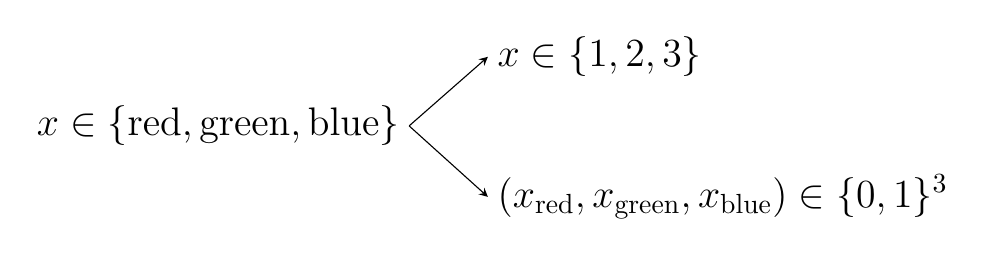
\begin{tikzpicture}[every node/.style={font={\Large}}]
			\node[anchor=east] (a) at (0, 0) {$x \in \{ \text{red}, \text{green}, \text{blue} \}$};
			\node[anchor=south west] (b) at (1, .5) {$x \in \{ 1, 2, 3 \}$};
			\node[red!85!black] (bmark) at (b.east) {\quad \huge \xmark};
			\node[anchor=north west] (c) at (1,-.5) {$(x_{\text{red}}, x_{\text{green}}, x_{\text{blue}}) \in \{ 0, 1 \}^3$};
			\node[green!75!black] (cmark) at (c.east) {\quad \huge \cmark};
			
			\path[-stealth]
			(a.east) edge (b.west) edge (c.west)
			;
		\end{tikzpicture}
	\end{center}
\end{frame}

	\section{The DGIM Algorithm}
	% !TeX spellcheck = en_GB
\begin{frame}{The Datar-Gionis-Indyk-Motwani Algorithm}
	\begin{block}{Objectives}
		\begin{itemize}
			\item
			\emphblack{Estimate} the number of \emphblack{ones} in a bit stream!

			\item
			Be \emphblack{space-efficient}!
		\end{itemize}
	\end{block}
	\begin{itemize}
		\item
		window size $N$

		\item
		$\mathcal{O}(\log_2 N)$ \emphblue{buckets}
		\begin{itemize}
			\item
			\emphblack{timestamp}

			\item
			\emphblack{size} = number of ones
			\begin{itemize}
				\item
				powers of two

				\item
				one or two of each size

				\item
				sizes never decreasing moving back
			\end{itemize}

			\item
			include all ones; end with ones
		\end{itemize}
	
		\item
		needs only \emphmathblack{\mathcal{O}( \!\!\:(\log_2 N)^2 )} \emphblack{bits}
	
		\item
		\emphblue{estimation}: half the size of the oldest bucket + sum of sizes of all other buckets
		\begin{itemize}
			\item
			error rate: 50\%
		\end{itemize}
	\end{itemize}
	%
	\vspace{1mm}
	%
	{
		\Large
		\begin{equation*}
			\mathtt{\boxed{\dots 1 ~ 0 ~ 1} ~ \boxed{1 ~ 0 ~ 1 ~ 1 ~ 0 ~ 0 ~ 0 ~ 1} ~ 0 ~ \boxed{1 ~ 1 ~ 1 ~ 0 ~ 1} ~ \boxed{1 ~ 0 ~ 0 ~ 1} ~ 0 ~ \boxed{1} ~ \boxed{1} ~ 0}
		\end{equation*}
	}
	%
	\begin{center}
		\small
		estimation:~16 \qquad\qquad reality:~14
	\end{center}
\end{frame}
	
	\section{The Mushroom Data Set}
	
	\section{The Implementation}

	\section{References}
	% !TeX spellcheck = en_GB
\begin{frame}{References}
	\begin{itemize}
		\item
		Project code:
		\url{https://github.com/s9770652/DS1-DGIM}
		
		\item
		Mushroom data set:
		\url{https://archive-beta.ics.uci.edu/ml/datasets/mushroom}
		
		\item
		Streamlit:
		\url{https://streamlit.io/}
		
		\item
		Python package \emph{dgim}:
		\url{https://pypi.org/project/dgim/}
		
		\item
		Description of one-hot encoding:
		\url{https://sherbold.github.io/intro-to-data-science/04_Data-Analysis-Overview.html\#Features}
		
		\item
		Description of the DGIM algorithm (Section 4.6):
		\url{http://infolab.stanford.edu/~ullman/mmds/ch4.pdf}
	\end{itemize}
\end{frame}
\end{document}